%%%%%%%%%%%%%%%%%%%%%%%%%%%%%%%%%%%%%%%%%
% Beamer Presentation
% LaTeX Template
% Version 1.0 (10/11/12)
%
% This template has been downloaded from:
% http://www.LaTeXTemplates.com
%
% License:
% CC BY-NC-SA 3.0 (http://creativecommons.org/licenses/by-nc-sa/3.0/)
%
%%%%%%%%%%%%%%%%%%%%%%%%%%%%%%%%%%%%%%%%%

%----------------------------------------------------------------------------------------
%	PACKAGES AND THEMES
%----------------------------------------------------------------------------------------

\documentclass[t]{beamer}

\mode<presentation> {

% The Beamer class comes with a number of default slide themes
% which change the colors and layouts of slides. Below this is a list
% of all the themes, uncomment each in turn to see what they look like.

%\usetheme{default}
%\usetheme{AnnArbor}
%\usetheme{Antibes}
%\usetheme{Bergen}
%\usetheme{Berkeley}
%\usetheme{Berlin}
%\usetheme{Boadilla}
%\usetheme{CambridgeUS}
%\usetheme{Copenhagen}
%\usetheme{Darmstadt}
%\usetheme{Dresden}
%\usetheme{Frankfurt}
%\usetheme{Goettingen}
%\usetheme{Hannover}
%\usetheme{Ilmenau}
%\usetheme{JuanLesPins}
%\usetheme{Luebeck}
\usetheme{Madrid}
%\usetheme{Malmoe}
%\usetheme{Marburg}
%\usetheme{Montpellier}
%\usetheme{PaloAlto}
%\usetheme{Pittsburgh}
%\usetheme{Rochester}
%\usetheme{Singapore}
%\usetheme{Szeged}
%\usetheme{Warsaw}

% As well as themes, the Beamer class has a number of color themes
% for any slide theme. Uncomment each of these in turn to see how it
% changes the colors of your current slide theme.

%\usecolortheme{albatross}
%\usecolortheme{beaver}
%\usecolortheme{beetle}
%\usecolortheme{crane}
%\usecolortheme{dolphin}
%\usecolortheme{dove}
%\usecolortheme{fly}
%\usecolortheme{lily}
%\usecolortheme{orchid}
%\usecolortheme{rose}
%\usecolortheme{seagull}
%\usecolortheme{seahorse}
%\usecolortheme{whale}
%\usecolortheme{wolverine}

%\setbeamertemplate{footline} % To remove the footer line in all slides uncomment this line
%\setbeamertemplate{footline}[page number] % To replace the footer line in all slides with a simple slide count uncomment this line

%\setbeamertemplate{navigation symbols}{} % To remove the navigation symbols from the bottom of all slides uncomment this line
}

\usepackage{graphicx} % Allows including images
\usepackage{booktabs} % Allows the use of \toprule, \midrule and \bottomrule in tables
\usepackage{fancyvrb} % Tabs in verbatim
%----------------------------------------------------------------------------------------
%	TITLE PAGE
%----------------------------------------------------------------------------------------

\title[uC101]{uC101: Introduction to Microcontrollers / Interfacing with the real world} % The short title appears at the bottom of every slide, the full title is only on the title page

\author{Josh Johnson} % Your name
\institute[] % Your institution as it will appear on the bottom of every slide, may be shorthand to save space
{ \\ % Your institution for the title page
\medskip
\textit{} % Your email address
}
\date{13/5/2019} % Date, can be changed to a custom date

\begin{document}

\begin{frame}
\titlepage % Print the title page as the first slide
\end{frame}

%----------------------------------------------------------------------------------------
%	PRESENTATION SLIDES
%----------------------------------------------------------------------------------------

\begin{frame}
\frametitle{Overview}
\begin{itemize}
\item Assembly of Hardware / Installation of Software
\item Microcontroller 101
\item Tools
\item Bit Math
\item Demos
\begin{itemize}
	\item Blink
	\item Button
	\item RGB LED (PWM)
	\item Rotary Encoder
	\item Charlieplexing
\end{itemize}
	

\end{itemize}
\vspace{20mm}
Project Files: \url{github.com/joshajohnson/CBRhardware}\\
\end{frame}

%----------------------------------------------------------------------------------------

\begin{frame}[t]
\frametitle{Assembly of Hardware}

\begin{figure}
	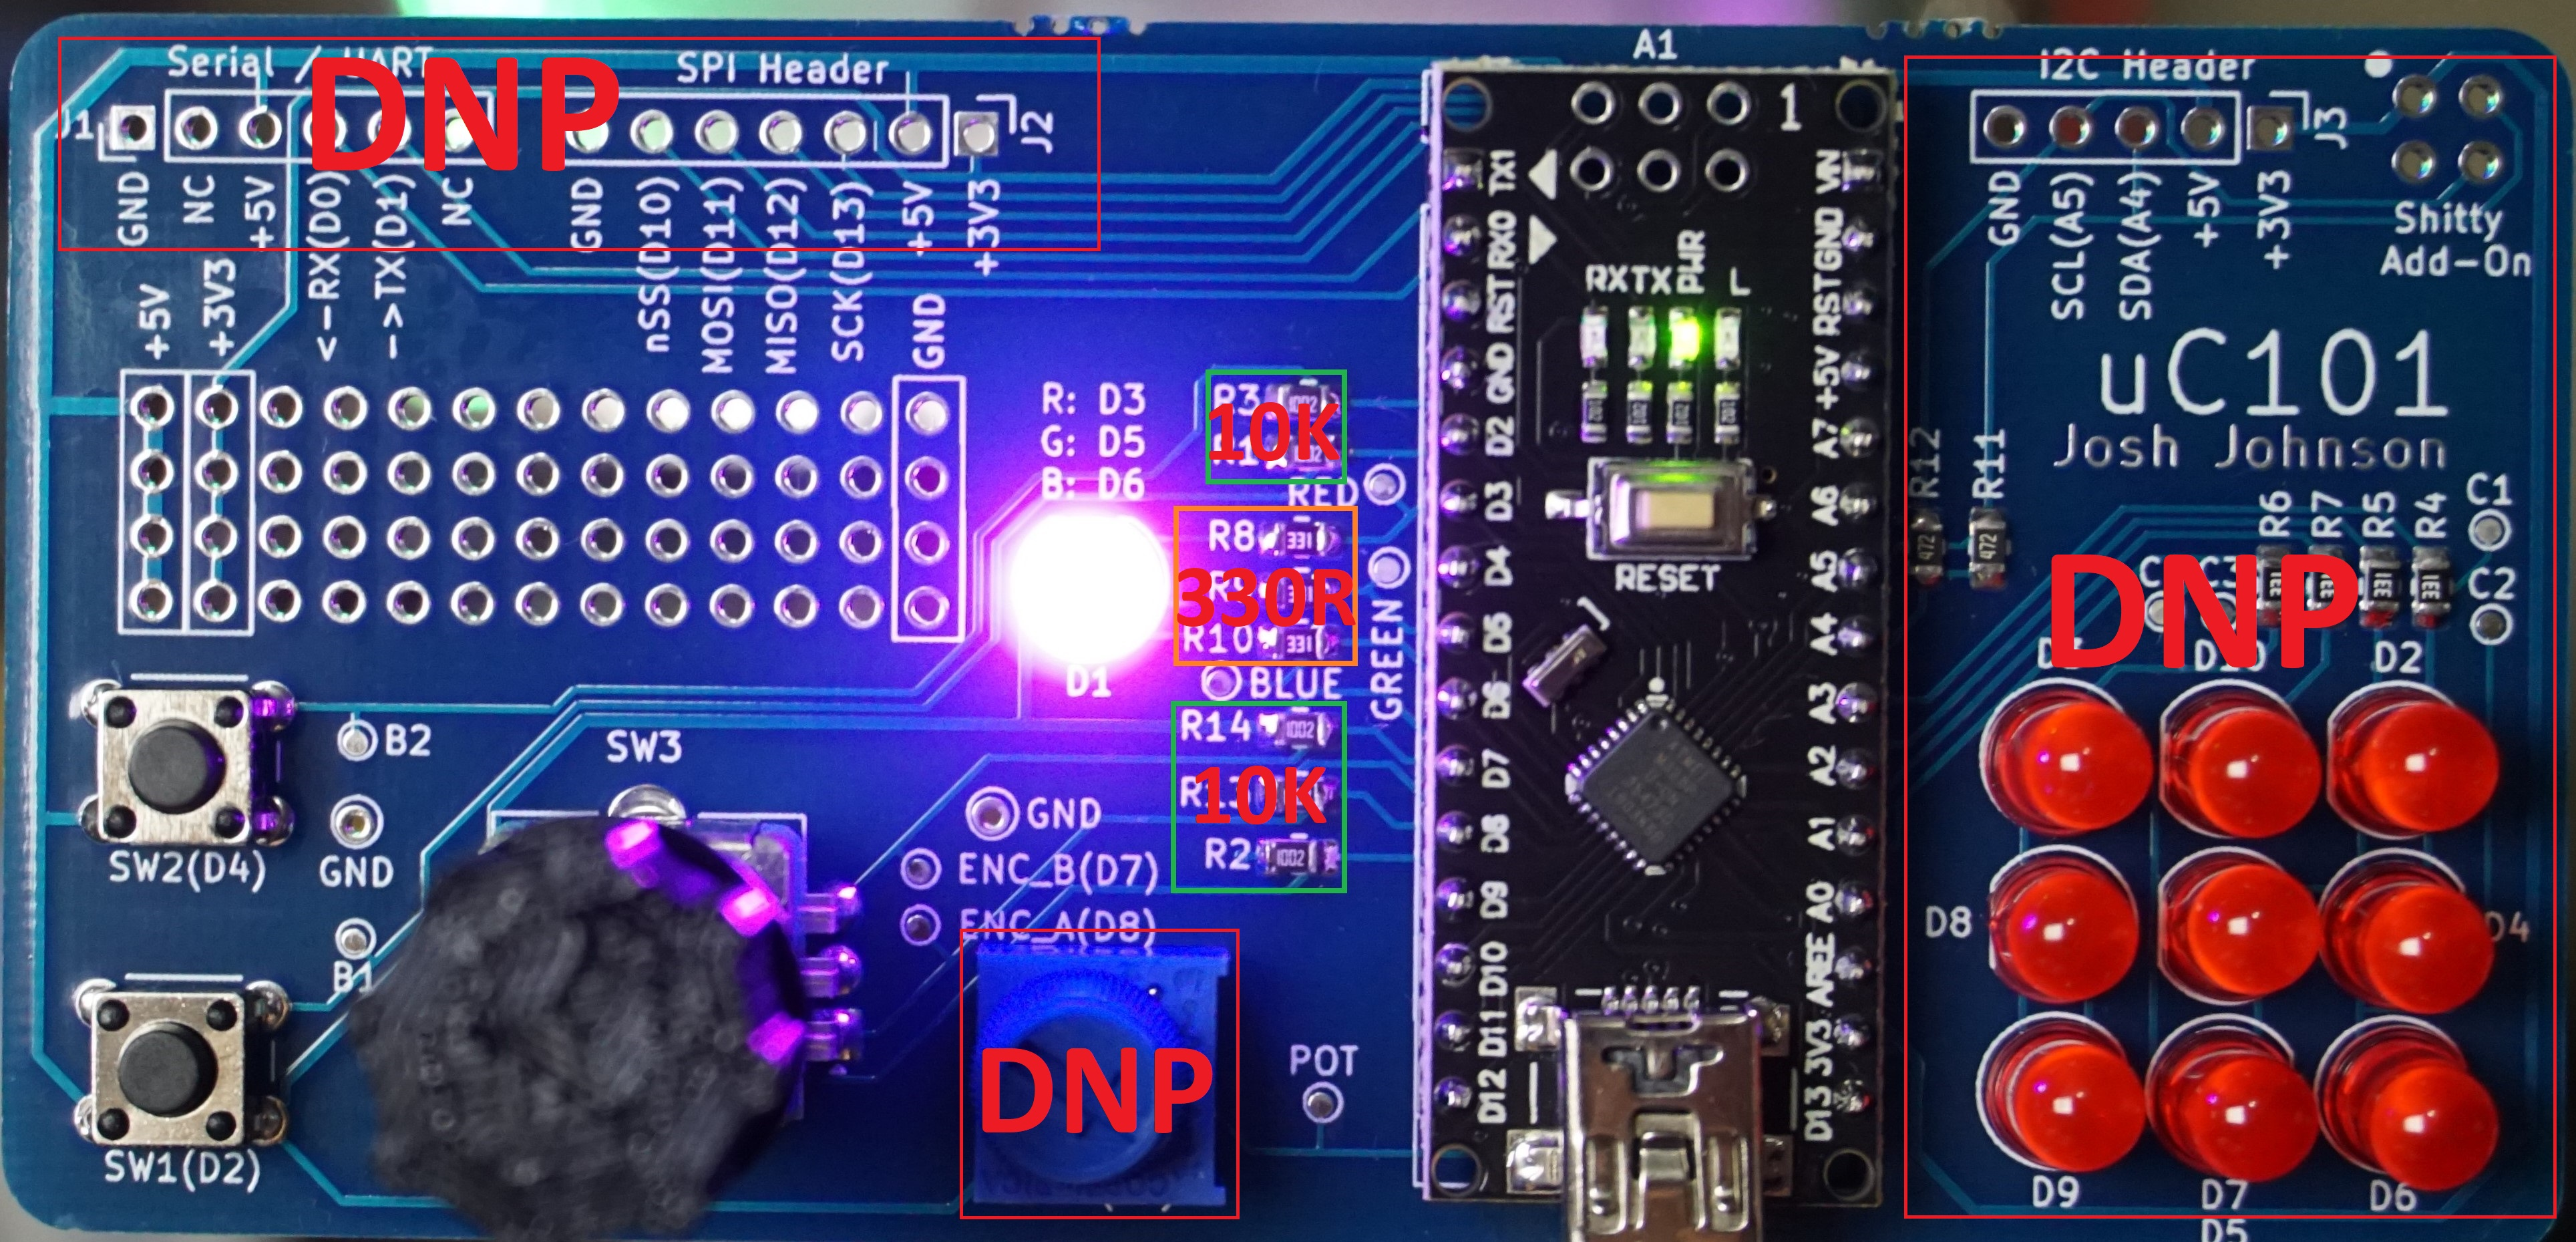
\includegraphics[width=1\linewidth]{hardware.JPG}
\end{figure}

\end{frame}

%----------------------------------------------------------------------------------------

%----------------------------------------------------------------------------------------

\begin{frame}[t]
\frametitle{Software Installation!}
Install Arduino  IDE\\
Copy the uC101Library folder to \texttt{/Arduino/libraries}\\
In Arduino IDE:\\
\texttt{File->Examples->uC101->blink}\\
\texttt{Tools->Board->Arduino Nano}\\
\texttt{Tools->Processor->ATmega328p} OR\\
\texttt{Tools->Processor->ATmega328p (Old Bootloader)}\\
\texttt{Tools->Port->\$comPort}\\
Run blink.ino and confirm that the onboard LED is blinking


\end{frame}

\begin{frame}[t]
\frametitle{Microcontroller 101}

\textbf{What is a microcontroller?} 

\begin{figure}
	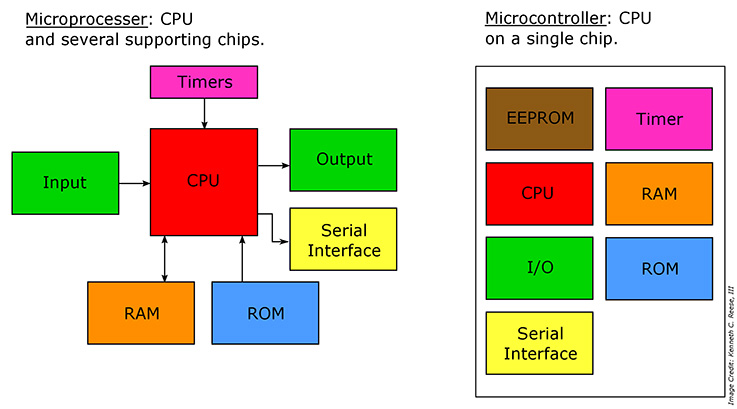
\includegraphics[scale=0.4]{microProcessorVsController.jpg}
\end{figure}

\end{frame}

%----------------------------------------------------------------------------------------

\begin{frame}[t]
\frametitle{Microcontroller 101}

\textbf{Common Options} 

\begin{columns}
	\column{.2\textwidth}
	8 bit
	\begin{itemize}
		\item ATtiny
		\item ATmega \\(Atmel / \\Microchip)
		\item PIC \\(Microchip)
	\end{itemize}

	\column{.2\textwidth}
	16 bit
	\begin{itemize}
		\item MSP430 (TI)
	\end{itemize}
	
	
	\column{.3\textwidth}
	32 bit
	\begin{itemize}
		\item STM32 (ST)
		\item SAM (Atmel/Microchip)
		\item nRF5x (Nordic Semi)
		\item ESP8266/32 (Espressif)
		\item CCxxxx (TI)
		\item LPCxxxx (NXP)
		\item PIC32 (Microchip)
	\end{itemize}

	\column{.29\textwidth}
	32 bit ARM cores
	\begin{itemize}
		\item Cortex-M0/M0+
		\item Cortex-M1 (FPGA only)
		\item Cortex-M3
		\item Cortex-M4 (M3 + DSP + FPU)
		\item ...
		
	\end{itemize}
	
\end{columns}

\end{frame}

%----------------------------------------------------------------------------------------


\begin{frame}[t]
\frametitle{Microcontroller 101}

\textbf{How to choose?}
\begin{itemize}
	\item Compute power
	\begin{itemize}
		\item 8 bit vs 32 bit
		\item DSP / FPU
	\end{itemize} 
	\item Peripherals 
	\begin{itemize}
		\item Wireless
			\begin{itemize}
			\item WiFi
			\item Bluetooth
			\item LoRa
			\item Cellular
		\end{itemize} 
		\item USB
		\item ADC
		\item Ethernet
		\item CAN
		\item Number of SPI/UART/I2C/Timers
	\end{itemize} 
	
\end{itemize} 



\end{frame}

%----------------------------------------------------------------------------------------

\begin{frame}[t]
\frametitle{Microcontroller 101}
\textbf{ATmega328p Architecture} 
\begin{figure}
	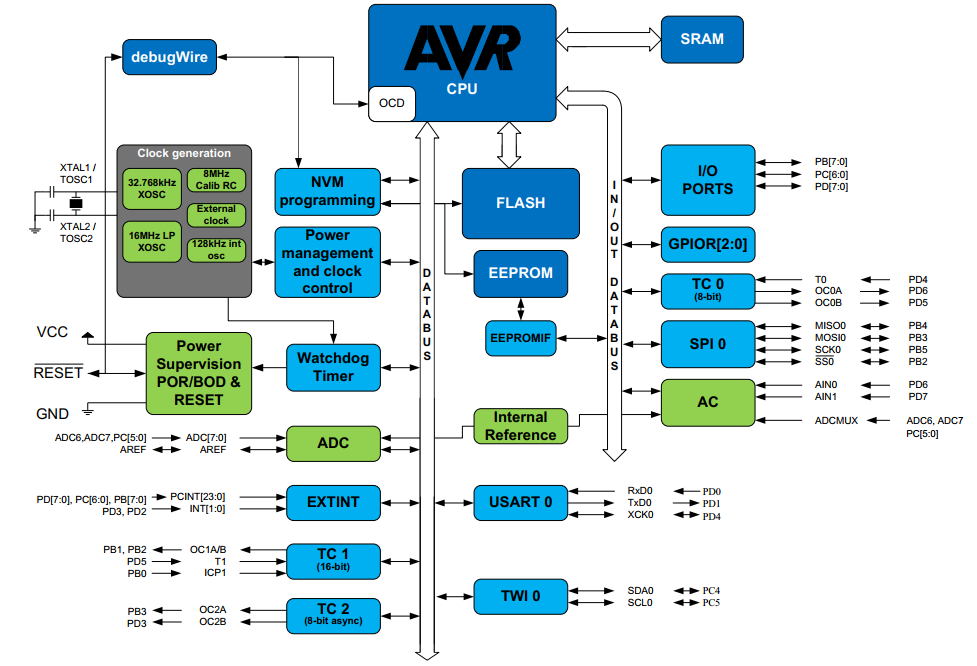
\includegraphics[scale=0.4]{328pArchitecture.PNG}
\end{figure}

\end{frame}


%----------------------------------------------------------------------------------------

\begin{frame}[t]
\frametitle{Tools}
\begin{itemize}
	\item Oscilloscope
	\begin{itemize}
		\item + High quality time domain measurements ($\ge$8 bits, $\ge$1 GSPS)
		\item - Expensive, short record time
	\end{itemize} 	
	\item Logic Analyser
	\begin{itemize}
		\item + Easy to use UI, long sample time / depth 
		\item - 1 bit*, low sample rate (25 - 100 - $\ge$500 MSPS)
		\item * some logic analysers have limited analog capabilities 
	\end{itemize} 
	\item Debugger
	\begin{itemize}
		\item Program and debug device
	\end{itemize} 
	\item Multimeter
	\begin{itemize}
		\item Voltage and resistance measurements
	\end{itemize} 
	\item Development Board
	\begin{itemize}
		\item Whilst not a tool, extremely helpful whilst bringing up firmware
		\item Helpful when developing code - the issue isn't (typically) the hardware!
	\end{itemize} 
\end{itemize} 
\end{frame}

%----------------------------------------------------------------------------------------

\begin{frame}[t,fragile]
\frametitle{Bitwise Operators}

\begin{figure}
	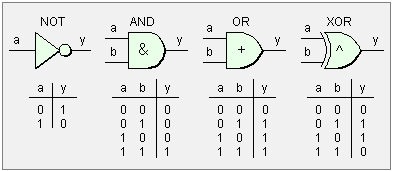
\includegraphics[scale=0.8]{truthTables.png}
\end{figure}

\begin{BVerbatim}[tabsize=1]
       y = ~a      y = a & b    y = a | b    y = a ^ b
               NOT y = a && b
\end{BVerbatim}

\end{frame}

%----------------------------------------------------------------------------------------

\begin{frame}[t,fragile]
\frametitle{Binary Operations}
Binary Numbers\\
\begin{verbatim}
Binary:   0  1  0  0  1  0  1  1
Weight: 128 64 32 16  8  4  2  1
Base 2  (Binary): 0b01001011
Base 10 (Decimal): 75 
Base 16 (Hexadecimal): 0x4B
\end{verbatim}

\break
Bit Shifting\\
\begin{verbatim}
a = 5;        // binary: 00000101
b = a << 3;   // binary: 00101000, 40 in decimal
c = b >> 3;   // binary: 00000101, back to 5 like we started
\end{verbatim}
\break
Putting it all together\\
\begin{verbatim}
x = 1;      // binary: 00000001
x <<= 3;    // binary: 00001000
x |= 3;     // binary: 00001011 - 3 is 11 in binary
x &= 1;     // binary: 00000001
\end{verbatim}
\end{frame}




%----------------------------------------------------------------------------------------

\begin{frame}[t,fragile]
\frametitle{Setting Registers}
\begin{columns}
\column{0.4\textwidth}
Setting a bit in a register
\begin{verbatim}
REG = REG | (1 << x);
REG |= (1<<x);
\end{verbatim}
Clearing a bit in a register
\begin{verbatim}
REG = REG & ~(1 << x);
REG &= ~(1<<x);
\end{verbatim}
Toggling a bit in a register
\begin{verbatim}
REG = REG ^ (1 << x);
REG ^= (1<<x);
\end{verbatim}
\column{0.59\textwidth}
Toggling multiple bits in a register
\begin{verbatim}
REG = REG ^ ((1 << x) | (1 << y));
REG ^= (1<<x) | (1<<y);
\end{verbatim}
AVR specific macro to bitshift
\begin{verbatim}
(1<<x) == _BV(x)
REG = (1<<x) | (1<<y);
REG = _BV(x) | _BV(y);
\end{verbatim}
What is the difference between the above and the first example (other than two variables)?
\end{columns}
\end{frame}
%----------------------------------------------------------------------------------------

\begin{frame}[t]
\frametitle{Demo Time!}
\begin{columns}
	\column{.6\textwidth}
	\begin{figure}
		
\includegraphics[scale=0.45]{thomasTankCode.jpg}
	\end{figure}	
	\column{.4\textwidth}
	\begin{itemize}
		\item I'm a hardware person, not a software person
		\item Solder is my preferred programming language
		\item I know enough to be dangerous, nothing more
		\item More experienced folks, please jump in and correct me / answer questions I can't / point out bad practices
		\item I'm here to learn like everyone else
	\end{itemize}
	
\end{columns}


\end{frame}

%----------------------------------------------------------------------------------------

\begin{frame}[t]
\frametitle{blink.ino}
\begin{itemize}
	\item Default blink
	\item Register level blink
	\item Nicer blink
	\item Even nicer blink
	\item Blink without delay
	\item Size comparison
	\item Speed comparison  
\end{itemize}
\end{frame}

%----------------------------------------------------------------------------------------

\begin{frame}[t]
\frametitle{button.ino}
\begin{itemize}
	\item Toggle on press
	\item Toggle on press with delay
	\item Button with interrupt
	\item Debounced button
\end{itemize}
\end{frame}

%----------------------------------------------------------------------------------------

\begin{frame}[t]
\frametitle{button.ino}
\textbf{Button Bounce}
\begin{itemize}
	\item What is button bounce?
	\item How to fix it? 
	\begin{itemize}
		\item Hardware - RC Circuit
		\item Hardware - RC + Schmitt trigger
		\item Software - Button polling
	\end{itemize}
\end{itemize}
\end{frame}

%----------------------------------------------------------------------------------------

\begin{frame}[t]
\frametitle{button.ino}
\textbf{Button Bounce}
\begin{itemize}
	\item What is button bounce?
\end{itemize}
\begin{figure}
	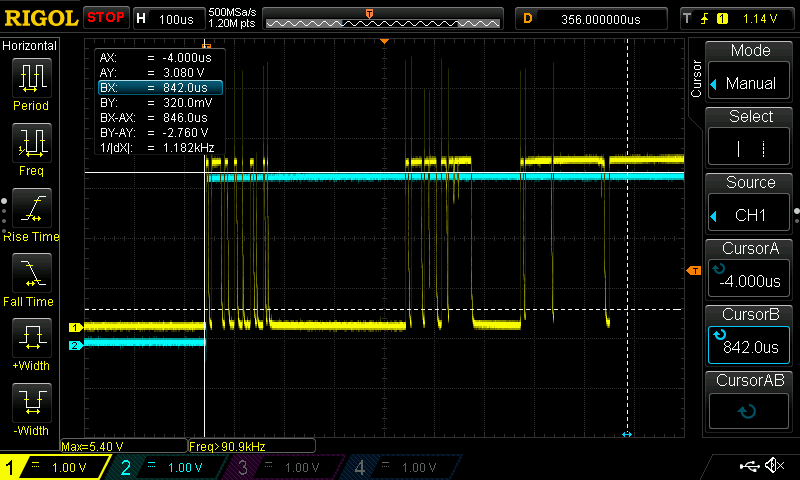
\includegraphics[scale=0.3]{bouncingBegin.png}
\end{figure}
\centering
Yellow = actual button, Blue = 'ideal button'

\end{frame}

%----------------------------------------------------------------------------------------

\begin{frame}[t]
\frametitle{button.ino}
\textbf{Button Bounce}
\begin{itemize}
	\item Fix 1 - RC Circuit
\end{itemize}
\begin{figure}
	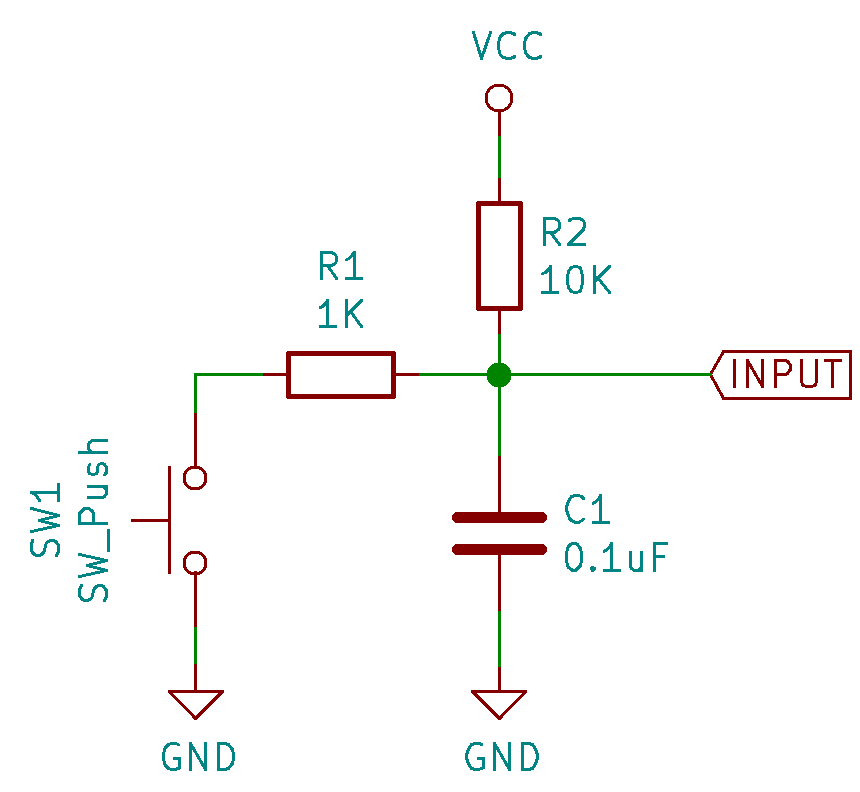
\includegraphics[scale=0.3]{RCswitch.PNG}
\end{figure}
\end{frame}

%----------------------------------------------------------------------------------------

\begin{frame}[t]
\frametitle{button.ino}
\textbf{Button Bounce}
\begin{itemize}
	\item Fix 2 - RC Circuit + Schmitt trigger
\end{itemize}
\begin{figure}
	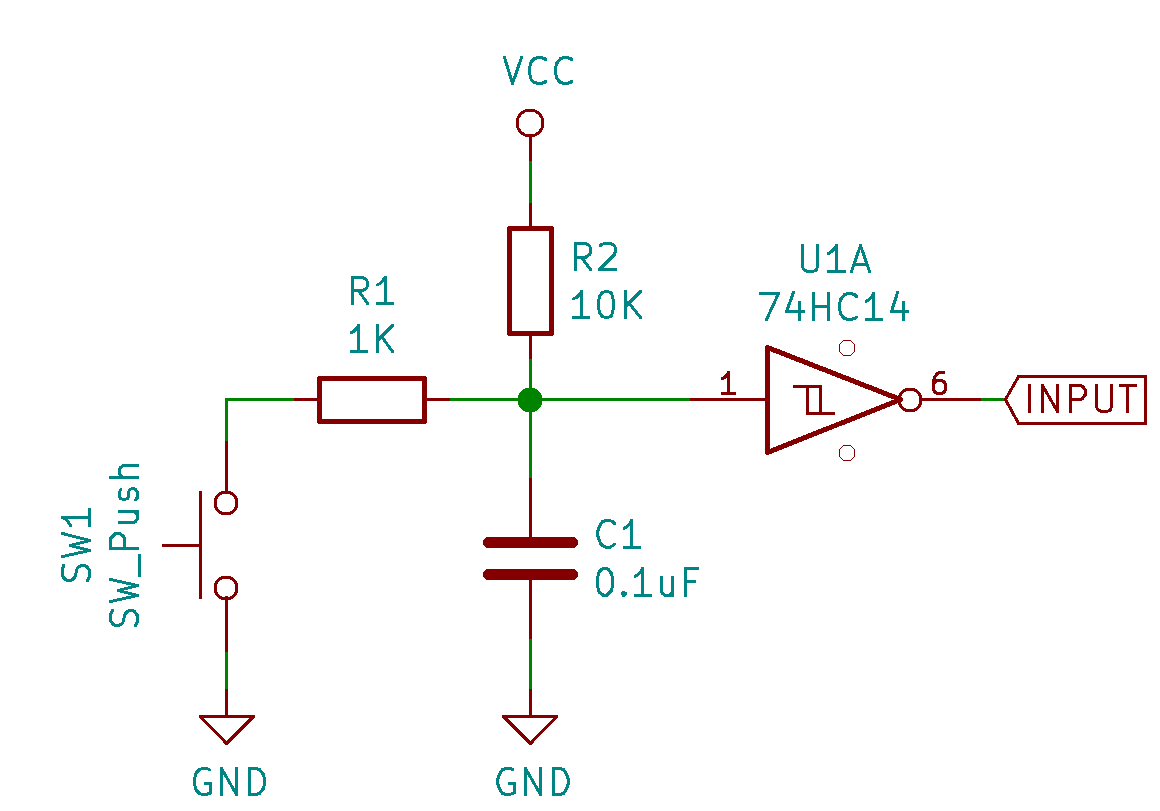
\includegraphics[scale=0.3]{schmittSwitch.PNG}
\end{figure}
\end{frame}

%----------------------------------------------------------------------------------------

\begin{frame}[t]
\frametitle{button.ino}
\textbf{Hysteresis}
\begin{figure}
	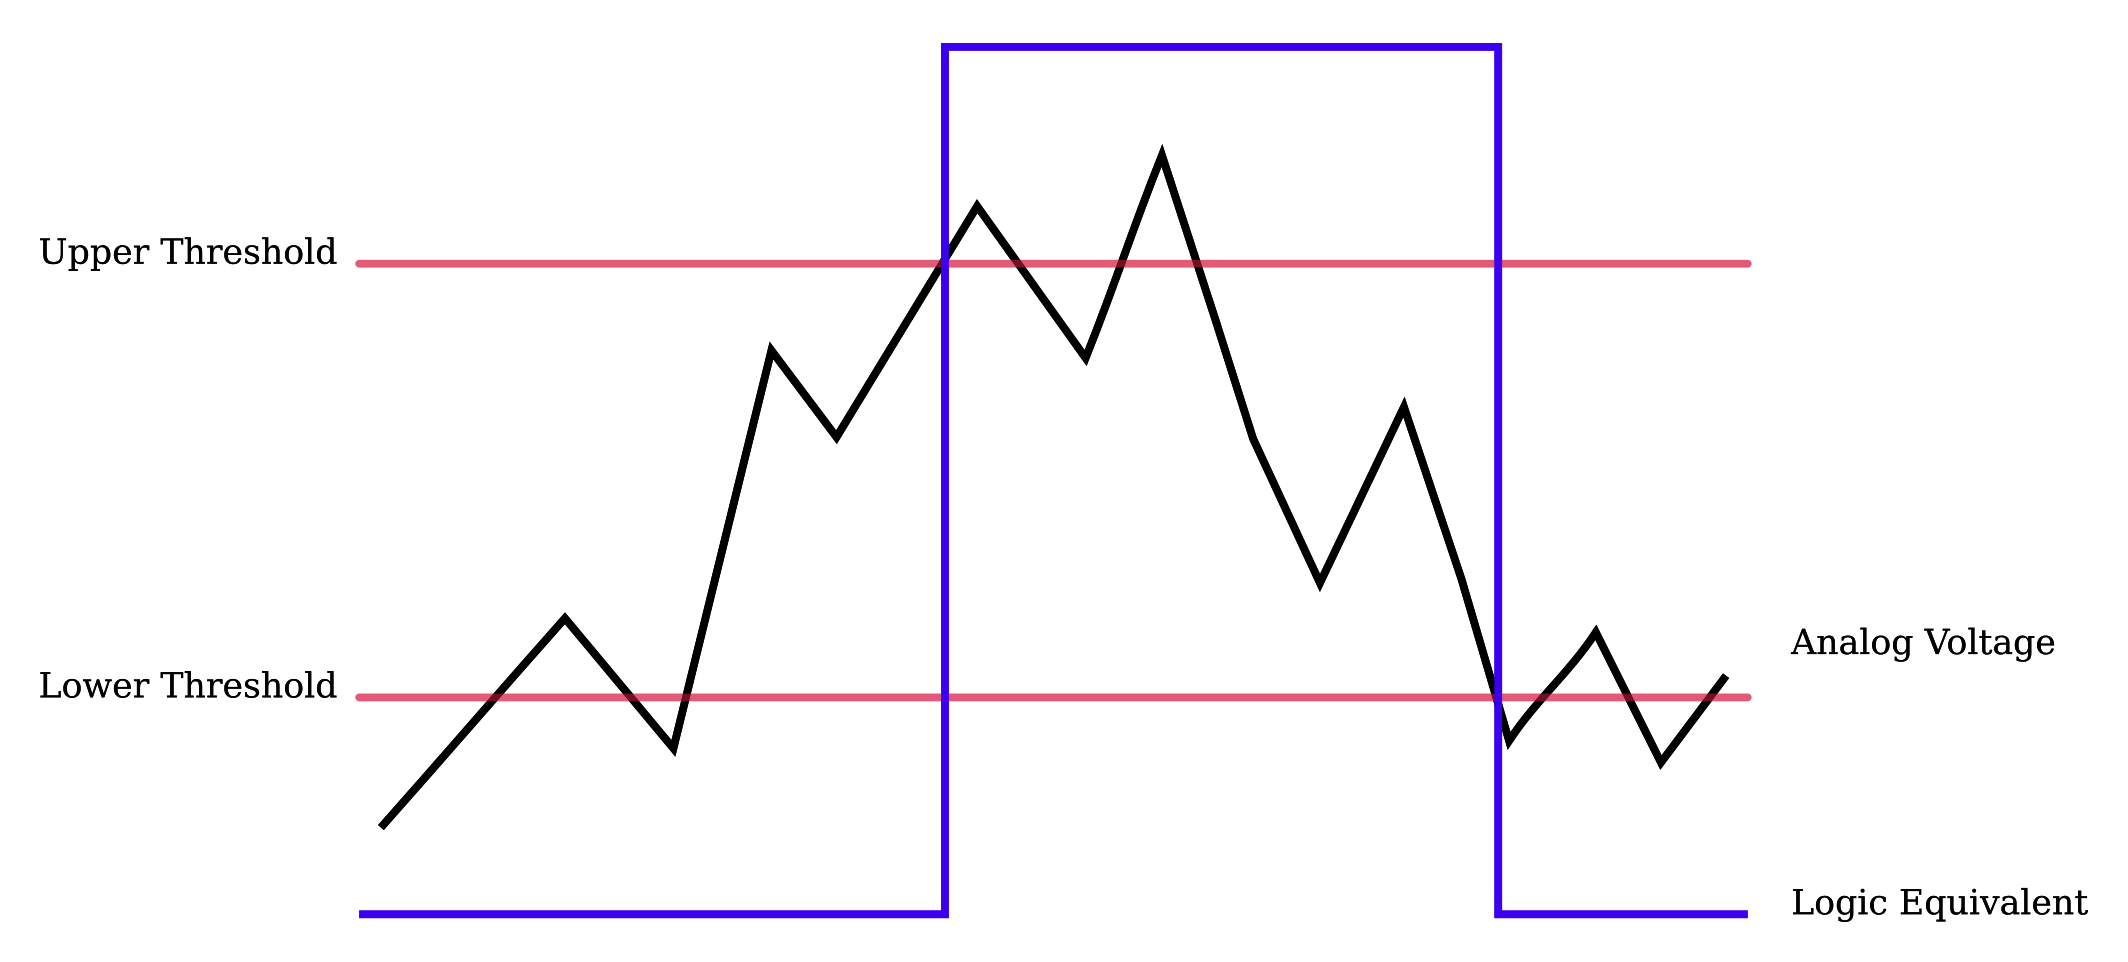
\includegraphics[scale=0.43]{hysteresis1.png}
\end{figure}
\end{frame}

%----------------------------------------------------------------------------------------

\begin{frame}[t]
\frametitle{button.ino}
\textbf{Button Bounce}
\begin{itemize}
	\item Fix 3 - Button polling (FPGA assignment version)
\end{itemize}
\begin{figure}
	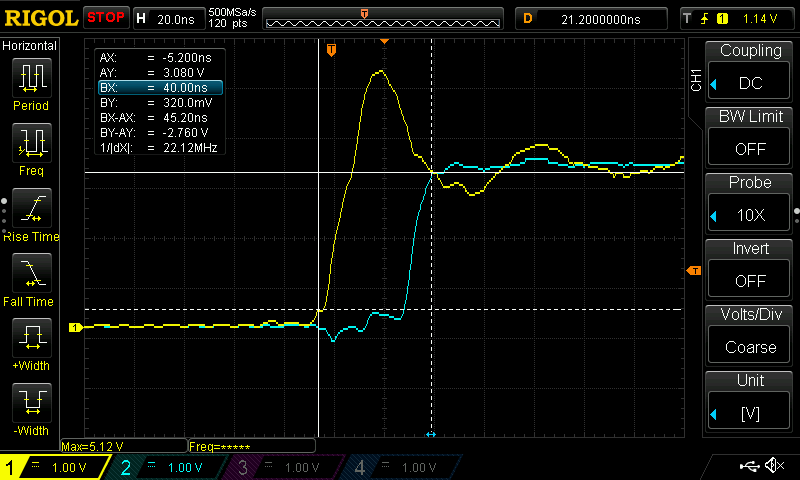
\includegraphics[scale=0.3]{riseDelay.png}
\end{figure}
\end{frame}

%----------------------------------------------------------------------------------------

\begin{frame}[t,fragile]
\frametitle{button.ino}
\textbf{Button Bounce}
\begin{itemize}
	\item Fix 3 - Button polling (uC101 version)
\end{itemize}
\begin{verbatim}
// Shift in a new value
history = history << 1;
history |= readPin(button);

// Check for button conditions
(history == 0b11111111) ? on = 1 : on = 0;
(history == 0b00000000) ? off = 1 : off = 0;
(history == 0b01111111) ? rising = 1 : rising = 0;
(history == 0b10000000) ? falling = 1 : falling = 0;
\end{verbatim}
Above code called every 1-5ms

\end{frame}

%----------------------------------------------------------------------------------------

\begin{frame}[t]
\frametitle{pwmLED.ino}
\textbf{Pulse Width Modulation}

\begin{figure}
	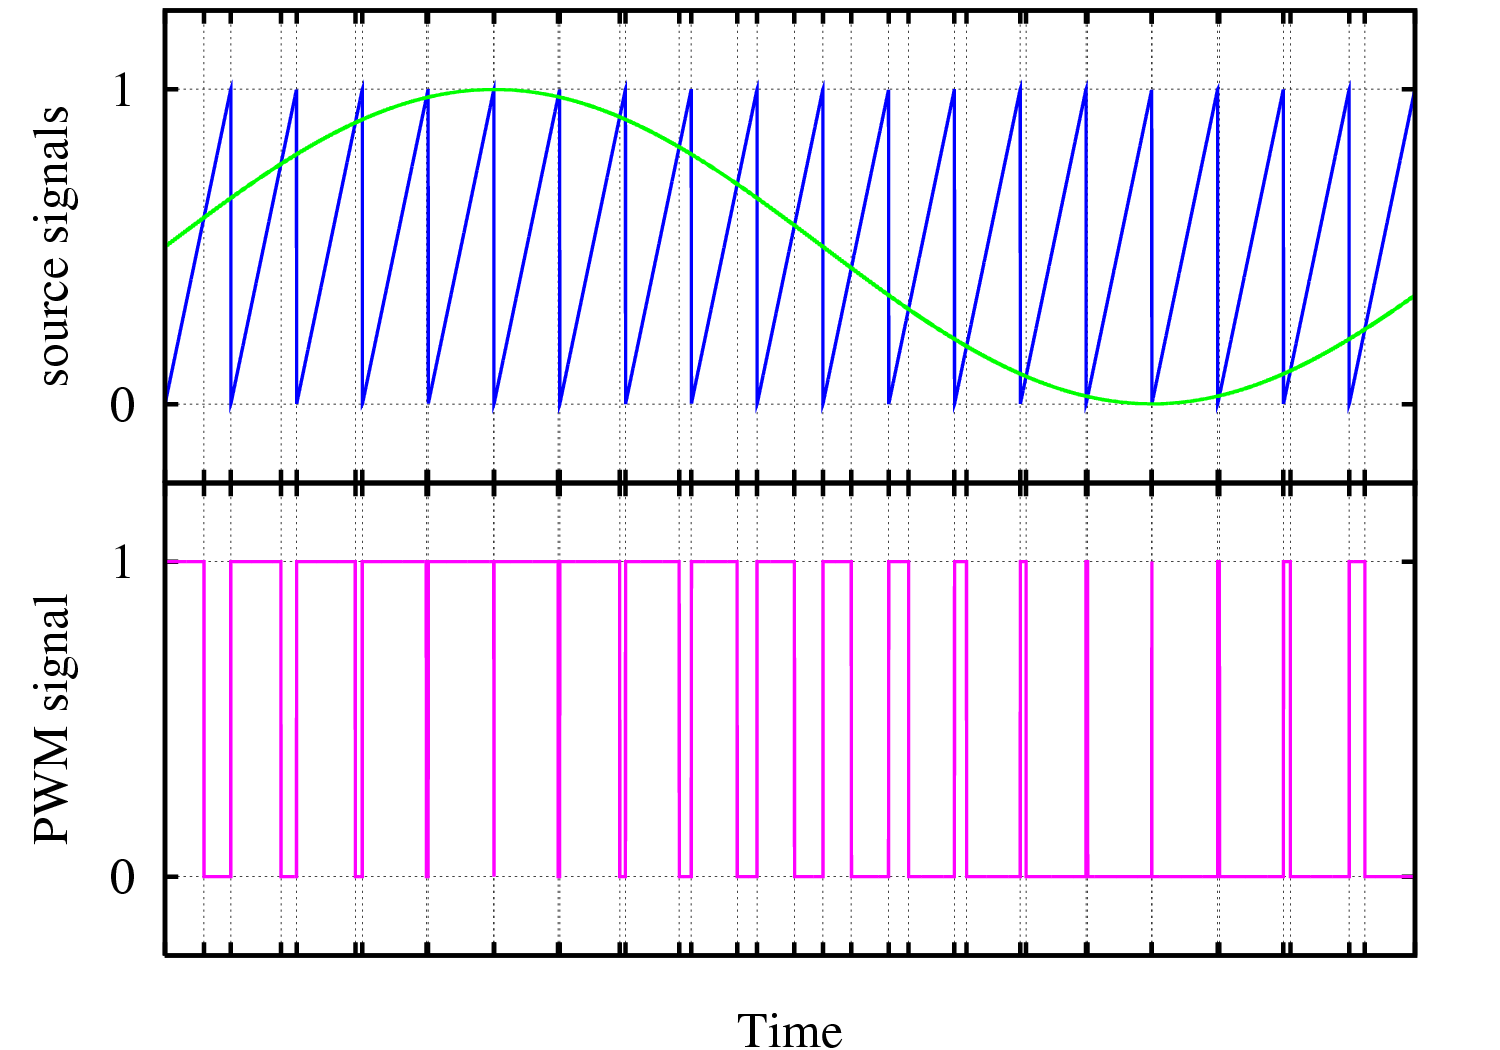
\includegraphics[width=0.8\textwidth]{pwm_wave.png}
\end{figure}


\end{frame}

%----------------------------------------------------------------------------------------

\begin{frame}[t,fragile]
\frametitle{rotaryEncoder.ino}
\textbf{Rotary Encoder Internal Operation}

\begin{figure}
	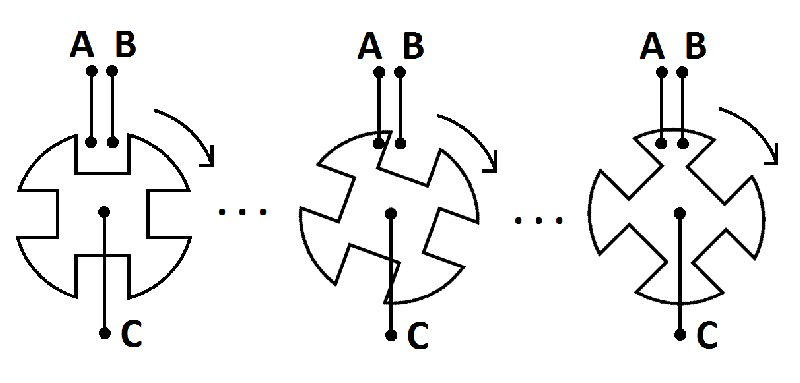
\includegraphics[width=0.8\textwidth]{encoderInternals.jpg}
\end{figure}


\end{frame}


%----------------------------------------------------------------------------------------

\begin{frame}[t]
\frametitle{rotaryEncoder.ino}
\textbf{Rotary Encoder Output}

\begin{figure}
	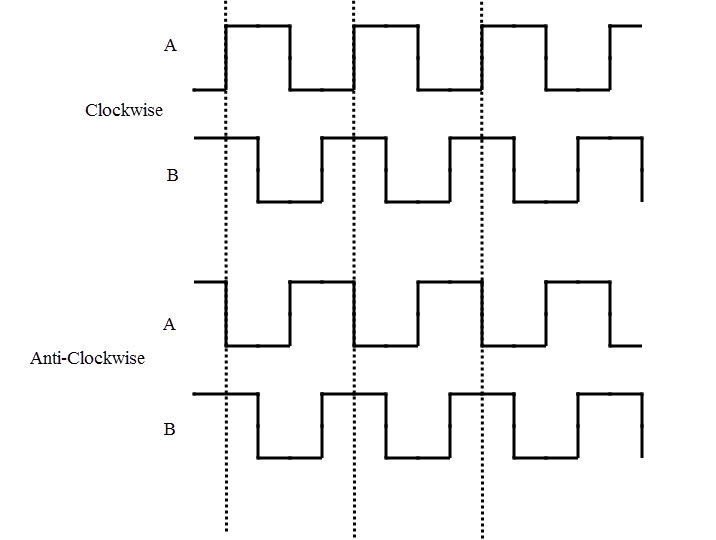
\includegraphics[width=0.8\textwidth]{Rotary-Encoder-Output.jpg}
\end{figure}


\end{frame}

%----------------------------------------------------------------------------------------

\begin{frame}[t,fragile]
\frametitle{rotaryEncoder.ino}
\textbf{Rotary Encoder Code}

\begin{verbatim}
(onB && risingA) ? clockwise = 1 : clockwise = 0;
(onB && fallingA) ? antiClockwise = 1 : antiClockwise = 0;
\end{verbatim}
or
\begin{verbatim}
(onB && risingA) ? clockwise = 1 : clockwise = 0;
(onA && risingB) ? antiClockwise = 1 : antiClockwise = 0;
\end{verbatim}
or
\begin{verbatim}
(fallingA && onB) ? clockwise = 1 : clockwise = 0;
(fallingA && offB) ? antiClockwise = 1 : antiClockwise = 0;
\end{verbatim}

all are functionally identical, however last one can be pin interrupt driven


\end{frame}

%----------------------------------------------------------------------------------------

\begin{frame}[t]
\frametitle{charlieplexing.ino}
\textbf{Charlieplexing vs Multiplexing}

\begin{figure}
	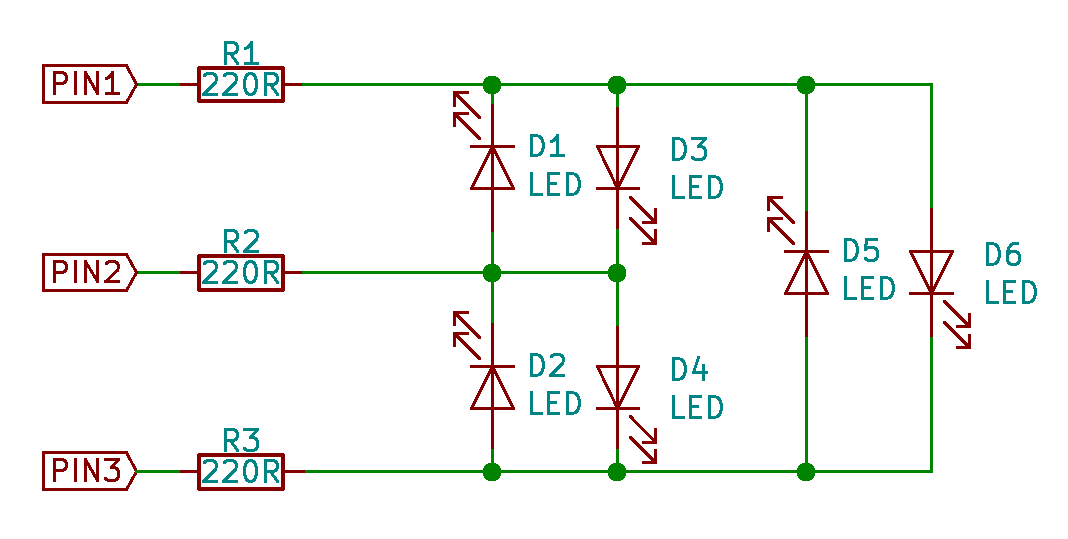
\includegraphics[width=0.8\textwidth]{charliePlexing.PNG}
\end{figure}
\centering
Charlieplexing: numLed = $p^2-p$ \\
Has to be scanned

\end{frame}

%----------------------------------------------------------------------------------------

\begin{frame}[t]
\frametitle{charlieplexing.ino}
\textbf{How to tristate a pin}

\begin{figure}
	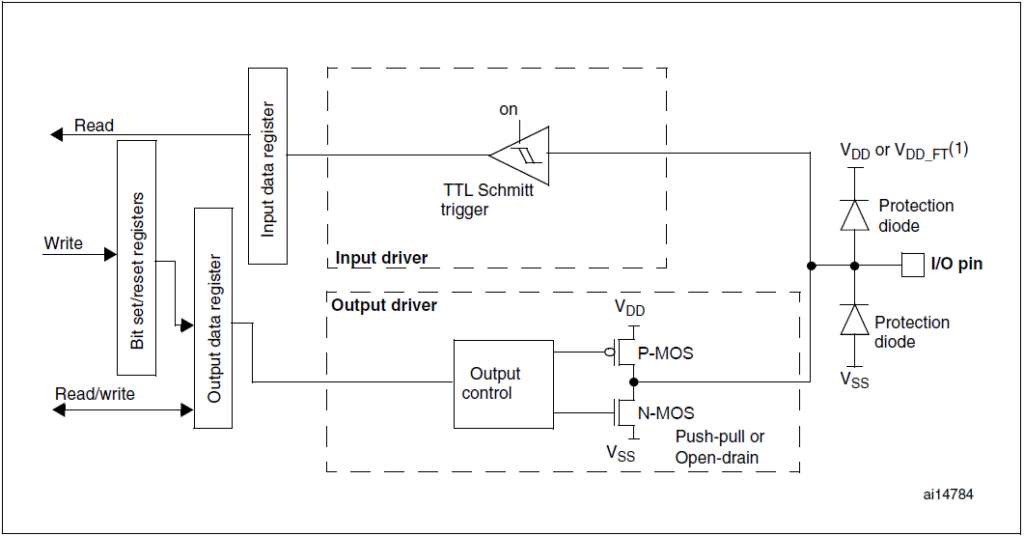
\includegraphics[width=0.8\textwidth]{gpioOutput.png}
\end{figure}


\end{frame}

%----------------------------------------------------------------------------------------

\begin{frame}[t]
\frametitle{charlieplexing.ino}
\textbf{How to tristate a pin}

\begin{figure}
	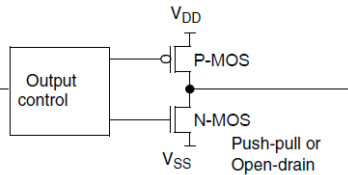
\includegraphics[width=0.8\textwidth]{gpioOutputClose.png}
\end{figure}

\end{frame}

%----------------------------------------------------------------------------------------

\begin{frame}[t]
\frametitle{charlieplexing.ino}
\textbf{Charlieplexing vs Multiplexing}

\begin{figure}
	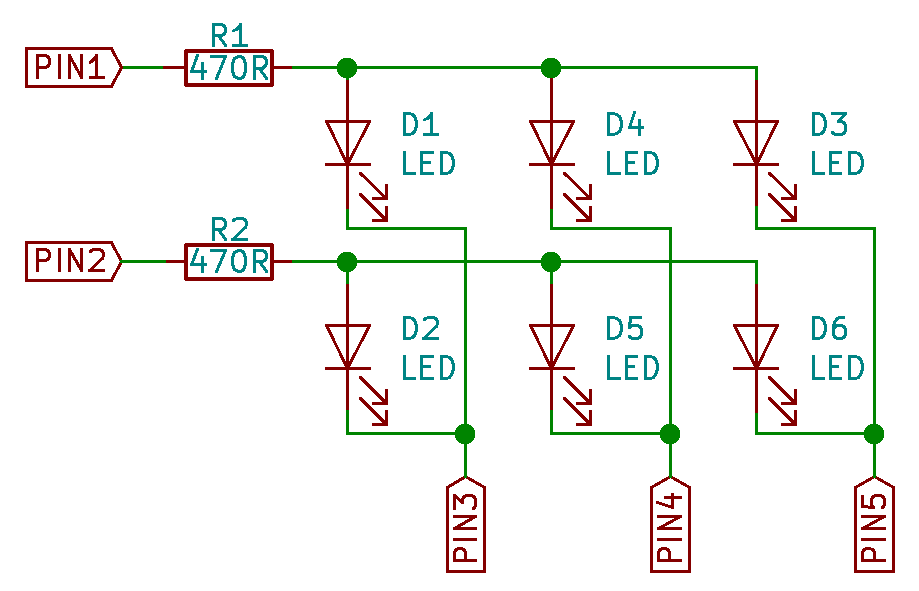
\includegraphics[width=0.7\textwidth]{multiPlexing.PNG}
\end{figure}
\centering
Multiplexing: numLed = $\left \lfloor{\frac{p}{2}^2}\right \rfloor$ \\
Can be continuously driven 

\end{frame}

%----------------------------------------------------------------------------------------


\begin{frame}
\frametitle{The End}
Links to resources: \texttt{uC101/README.md}
\vspace{5mm}

\textbf{Next month}
\begin{itemize}
	\item Breadboard to Printed Circuit Board
	\item Mechanical Design Considerations	
\end{itemize}
\vspace{3mm}
\textbf{Month after that}
\begin{itemize}
	\item uC102: Communication Protocol Edition	
\end{itemize}

\vspace{5mm}
Say Hello! \\
BSidesCbr Slack: josh\\
Twitter:  @\textunderscore joshajohnson\\
Email: josh@joshajohnson.com\\
\vspace{4mm}

Project Files: \url{github.com/joshajohnson/CBRhardware}\\\end{frame}


\end{document} 